\documentclass{article}
\usepackage{graphicx} % Required for inserting images
\usepackage[ngerman]{babel}
\usepackage{hyperref}
\usepackage{amsmath}
\usepackage{amssymb}

\title{Abgabe 1 für Computergestützte Methoden}
\author{Gruppe 38, Yasin Özdemir(4279187), \\Chris Giesbrecht(4111019), Levi Giesbrecht(4268836)}
\date{2. Dezember.2024}

\begin{document}
\maketitle
\tableofcontents
\newpage

\section{Der Zentrale Grenzwertsatz}
Der zentrale Grenzwertsatz (ZGS) ist ein fundamentales Resultat der Wahrscheinlichkeitstheorie, das die Verteilung von Summen unabhängiger, identisch verteilter $(i.i.d.)$ Zufallsvariablen (ZV) beschreibt. Er besagt, dass unter bestimmten Voraussetzungen die Summe einer großen Anzahl  solcher ZV annähernd normalverteilt ist, unabhängig von der Verteilung der einzelnen ZV. Dies ist besonders nützlich, da die Normalverteilung gut untersucht und mathematisch handhabbar ist.



\subsection{Aussage}
Sei $X_1, X_2, . . . , X_n$ eine Folge von $i.i.d.$ ZV mit dem Erwartungswert $\mu =\mathbb{E}(X_i)$ und der Varianz $\sigma^2 = Var(X_i)$, wobei  $0<\sigma^2<\infty$  gelte. Dann konvergiert die standardisierte Summe $Z_n$ dieser ZV für $n\rightarrow\infty$ in Verteilung gegen eine Standardnormalverteilung\footnote{Der zentrale Grenzwertsatz hat verschiedene Verallgemeinerungen. Eine davon ist der \textbf{Lindenberg-Feller-Zentrale-Grenzwertsatz}[\cite{AchimKlenke},Seite 328],der schwächere Bedingungen an die Unabhängigkeit und die identische Verteilung der ZV stellt.}

\begin{equation}
\label{eq:ZGS}    
Z_n=\frac{\sum\nolimits_{i=1}^n X_i-n\mu}{\sigma\sqrt{n}}\xrightarrow{d} \mathcal{N}(0,1)
\end{equation}
Das bedeutet, dass für große $n$ die Summe der ZV näherungsweise normalverteilt ist mit Erwartungswert $n\mu$ und Varianz $n\sigma^2$

\begin{equation}
\label{eq:ZGSs}
\sum_{i=1}^{n}X_i\sim \mathcal{N}(n\mu,n\sigma^2)
\end{equation}

\subsection{Erklärung der Standardisierung}

Um die Summe der ZV in eine Standardnormalverteilung zu transformieren, subtrahiert man den Erwartungswert $n\mu$ und teilt durch die Standardabweichung $\sigma\sqrt{n}$. Dies führt zu der obigen Formel (1). Die Darstellung (2) ist für $n\rightarrow\infty$ nicht wohl definiert. 




\subsection{Anwendung}
Der ZGS wird in vielen Bereichen der Statistik und der Wahrscheinlichkeitstheorie angewendet. Typische Beispiele sind: 
\begin{itemize}
    \item Hypothesentests 
    \item Statistische Stichprobenanalyse
\end{itemize}


\newpage
\section{Bearbeitung zur Aufgabe 1}
\subsection{Datenverarbeitung}
Nach dem Öffnen der Daten fällt auf, dass der Datensatz sehr unordentlich dargestellt wird. Um mit den gegebenen Daten arbeiten zu können importieren wir diese in eine Tabellenkalkulation, in unserem Fall in Excel. Dies tun wir indem wir den Datensatz downloaden und mit Excel öffnen.
Um uns einen besseren Überblick zu verschaffen, trennen wir die Daten nach Komma. Dies können wir realisieren indem wir A markieren und auf der Registerkarte auf Daten klicken und dann auf Text in Spalten. Um jetzt die höchste mittlere Temperatur zu ermitteln, nutzen wir die Formel

$$=MAX(J2;J36440)$$
Wir erhalten den Wert 83. Dadurch, dass unsere Temperatur in Fahrenheit gegeben ist, wollen wir diese in Grad Celsius umrechnen. Dies können wir mit der Formel: $$=(83-32)*5/9$$ daraus ergibt sich 28,3 Grad Celsius.

\subsection{Datenhaltung}
Die 1.Normalform wird erfüllt, indem nicht-atomare Attribute aufgeteilt werden, sodass sie ausschließlich einen unteilbaren Wert enthalten.

\begin{figure}[htbp]
    \hspace{-2.5cm}
    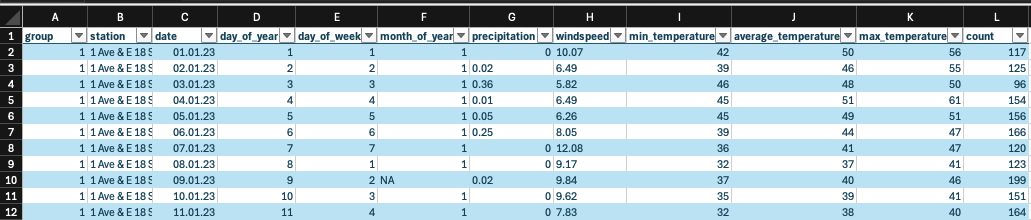
\includegraphics[width=1.5\linewidth]{Normalform 1.png}
    \caption{1. Normalform}
    \label{fig:enter-label}
\end{figure}
\newpage

Damit die 2.Normalform erfüllt ist, muss die 1.Normalform bereits gegeben sein. Danach werden die Tabellen in mehrere  Tabellen aufgeteilt und Fremdschlüssel-Beziehung werden hinzugefügt mit den passenden Abhängigkeiten dazu. 

\begin{figure}[htbp]
    \centering
    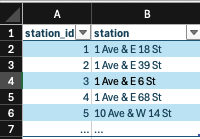
\includegraphics[width=0.5\linewidth]{Station id1.png}
    \caption{stationid}
\end{figure}

\begin{figure}[htbp]
    \hspace{-2.5cm}
    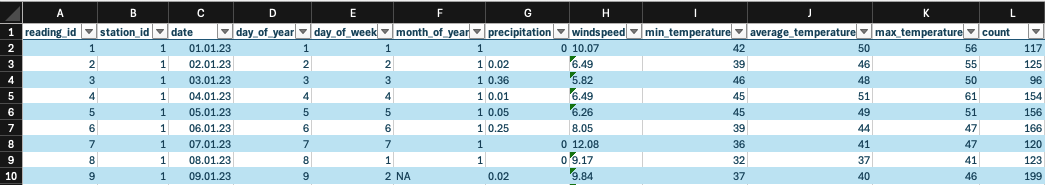
\includegraphics[width=1.5\linewidth]{Normalform2.png}
    \caption{2. Normalform}
\end{figure}


\newpage

\bibliographystyle{plain}
\bibliography{references}




Github Link:\\
\url{https://github.com/yasin1108/Abgabe1_COMET_WiSe2425_Gruppe38.pfd.git}

      
\end{document}